\chapter{Perzeptron-Implementierung in Python}\label{appendix:pythonperzeptron}

Wie bereits in Abschnitt~\ref{seq-mcpbool} für das MCP-Neuron gezeigt, wollen wir auch mit dem Rosenblatt-Perzeptron boolesche Funktionen nachbilden.\\

Das folgende Beispiel bezieht sich auf die \textbf{AND}-Funktion (vgl. Tabelle~\ref{tab:and}).

Zunächst definieren wir zwei Mengen $M_+$ und $M_-$: Für Elemente in $M_+$ ist die erwartete Ausgabe $1$, für Elemente in $M_-$ ist sie $0$ (vgl. Abbildung~\ref{fig-rpand}):

\begin{equation}
    M_+ \coloneqq \{(1, 1)\}\\
\end{equation}

\begin{equation}
    M_- \coloneqq \{(0, 0), (0,1), (1,0)\}
\end{equation}

\begin{figure}[h]
    \begin{center}
    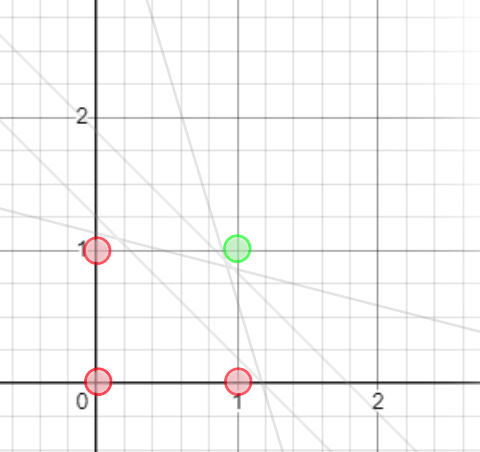
\includegraphics{chapters/Anhang/images/perceptron-and}
    \caption{Geometrische Interpretation der Perzeptron-Funktion im $\mathbb{R}^2$ (Quelle: Eigene Darstellung)}
    \end{center}
    \label{fig-rpand}
    \small {
    Die Abbildung zeigt alle möglichen zweiwertigem Interpretation von $A \land B$ in einem kartesischen Koordinatensystem.
    Offensichtlich ist die Anzahl der möglichen Trenngeraden (einige hier grau eingezeichnet) im $\mathbb{R}^2$ unendlich.
    }
\end{figure}

\pagebreak
Für unsere Perzeptron-Implementierung in Python\footnote{
    vollständiger Quellcode unter \url{https://github.com/ThorstenSuckow/pylabs} (abgerufen 25.08.2023)
} implementieren wir die Lernregel wie folgt:


\begin{lstlisting}[language=Python]
    for epoch in range(epochs):

        errors = 0

        for i in range(n):
            expected = y[i]
            net = X[i] @ self.w + self.bias
            result = self.heaviside(net)
            error = 0

            if result != expected:
                error = expected - result

                self.w += (X[i] * learning_rate * error)
                self.bias += learning_rate * error
\end{lstlisting}

\noindent
Der Algorithmus erhält eine vorgegebene Zahl von Epochen, in denen eine vollständige Konvergenz erwartet wird.
Innerhalb einer Epoche werden alle \verb|n| Trainingsdaten (enthalten in \verb|X|) durchgegangen.
In \verb|y| finden wir die erwartete Klassifizierung der Trainingsdaten:
Ist \verb|X[i] = [1,1]|, entspricht \verb|y[i] = 1| (vgl. Gleichung~\ref{eq:gl-expnet}).
\verb|net| entspricht dem Ergebnis von Gleichung~\ref{eq:gl-net}, und das Ergebnis \verb|result| der \textbf{Heaviside}-Funktion mit

\begin{equation}
    exp = \begin{cases}
              1 \text{ falls } \text{net} \geq 0 \\
              0 \text{ sonst}
    \end{cases}
    \label{eq:gl-expnet}
\end{equation}

\noindent
Die Lernregel wird so lange durchlaufen, bis für alle Trainingsdaten kein Fehler \verb|error| mehr auftritt oder alle Epochen ausgeschöpft sind.\\

\noindent
Der Algorithmus nutzt folgende Nomenklatur:\\


$\eta \coloneqq 1 \space \space \text{ (Lernrate)}$

$b \coloneqq 0 \space \space \text{ (Bias)}$\\

$w \coloneqq \begin{pmatrix}
          1 \\
          1
\end{pmatrix}\space \space \text{ (Gewichtsvektor)}$
\\
\\

$M_+ \coloneqq \{(1, 1)\}$

$M_- \coloneqq \{(0, 0), (0,1), (1,0)\}$

$net = w_1x_1 + w_2x_2 + b$\\

$exp = \begin{cases}
           1 \text{ falls } (x_1, x_2) \in M_+ \\
           0 \text{ sonst }
\end{cases}  \space \space \text{ (erwartete Ausgabe)}$
\\
\\

$res =  \begin{cases}
            0 \text{ falls } net < 0 \\
            1 \text{ sonst }
\end{cases}  \space \space \text{ (berechnete Ausgabe)}$\\

$err = exp - res  \space \space \text{ (Fehler)}$

$w^u = w + (x_1, x_2) * \eta * err  \space \space \text{ (aktualisierter Gewichtsvektor)}$

$b^u = b + \eta * err \space \space \text{ (aktualisierter Bias)}$\\


\noindent
Mit der o.a. Implementierung konvergiert das Perzeptron innerhalb von 5 Epochen.
In jeder Epoche werden 4 einzelne Daten trainiert, was insgesamt einer Anzahl von 20 Trainingsschritten entspricht.
Das Perzeptron hat also für $w_1$, $w_2$ Werte gefunden, so dass die folgenden 4 Ungleichungen gleichzeitig erfüllt sind:\\



$w_10 + w_20 < \Theta$\\

$w_11 + w_20 < \Theta$\\

$w_10 + w_21 < \Theta$\\

$w_11 + w_21 \geq \Theta$\\



Die folgenden Tabellen zeigen die Anpassungen im Detail.
Die geometrische Darstellung hierzu findet sich in Abbildung~\ref{fig-rp-and-epochs}.

\setlength{\tabcolsep}{0.8em}
\begin{table} %[hbtp]
    \centering
    \begin{tabular}{c | c | c | c | c | c | c | c | c | c | c | c | c}
        Epoche & $x_1$ & $x_2$ & $w_1$ & $w_2$ & $b$ & $net$ & $exp$ & $res$ & $err$ & $w^u_1$ & $w^u_2$ & $b^u$ \\
        \hline
        1.1& 0     & 0     & 1     & 1     & 0   & 0     & 0     & 1     & -1  & 1       & 1       & -1 \\
        1.2& 1     & 0     & 1     & 1     & -1  & 0     & 0     & 1     & -1  & 0       & 1       & -2 \\
        1.3& 0     & 1     & 0     & 1     & -2  & -1    & 0     & 0     & 0   & 0       & 1       & -2 \\
        1.4& 1     & 1     & 0     & 1     & -2  & -1    & 1     & 0     & 1   & 1       & 2       & -1 \\
    \end{tabular}
    \caption{Epoche 1 für \textbf{AND}}
    \label{tab:mcp-andep1}
\end{table}

\setlength{\tabcolsep}{0.8em}
\begin{table} %[hbtp]
    \centering
    \begin{tabular}{c | c | c | c | c | c | c | c | c | c | c | c | c}
        Epoche & $x_1$ & $x_2$ & $w_1$ & $w_2$ & $b$ & $net$ & $exp$ & $res$ & $err$ & $w^u_1$ & $w^u_2$ & $b^u$ \\
        \hline
        2.1& 0     & 0     & 1     & 2     & -1  & -1    & 0     & 0     & 0   & 1       & 2       & -1    \\
        2.2& 1     & 0     & 1     & 2     & -1  & 0     & 0     & 1     & -1  & 0       & 2       & -2    \\
        2.3& 0     & 1     & 0     & 2     & -2  & 0     & 0     & 1     & -1  & 0       & 1       & -3    \\
        2.4& 1     & 1     & 0     & 1     & -3  & -2    & 1     & 0     & 1   & 1       & 2       & -2    \\
    \end{tabular}
    \caption{Epoche 2 für \textbf{AND}}
    \label{tab:mcp-andep2}
\end{table}

\setlength{\tabcolsep}{0.8em}
\begin{table} %[hbtp]
    \centering
    \begin{tabular}{c | c | c | c | c | c | c | c | c | c | c | c | c}
        Epoche & $x_1$ & $x_2$ & $w_1$ & $w_2$ & $b$ & $net$ & $exp$ & $res$ & $err$ & $w^u_1$ & $w^u_2$ & $b^u$ \\
        \hline
        3.1& 0     & 0     & 1     & 2     & -2  & -2    & 0     & 0     & 0   & 1       & 2       & -2    \\
        3.2& 1     & 0     & 1     & 2     & -2  & -1    & 0     & 0     & 0   & 1       & 2       & -2    \\
        3.3& 0     & 1     & 1     & 2     & -2  & 0     & 0     & 1     & -1  & 1       & 1       & -3    \\
        3.4& 1     & 1     & 1     & 1     & -3  & -1    & 1     & 0     & 1   & 2       & 2       & -2    \\
    \end{tabular}
    \caption{Epoche 3 für \textbf{AND}}
    \label{tab:mcp-andep3}
\end{table}


\setlength{\tabcolsep}{0.8em}
\begin{table} %[hbtp]
    \centering
    \begin{tabular}{c | c | c | c | c | c | c | c | c | c | c | c | c}
        Epoche & $x_1$ & $x_2$ & $w_1$ & $w_2$ & $b$ & $net$ & $exp$ & $res$ & $err$ & $w^u_1$ & $w^u_2$ & $b^u$ \\
        \hline
        4.1& 0     & 0     & 2     & 2     & -2  & -2    & 0     & 0     & 0   & 2       & 2       & -2    \\
        4.2& 1     & 0     & 2     & 2     & -2  & 0     & 0     & 1     & -1  & 1       & 2       & -3    \\
        4.3& 0     & 1     & 1     & 2     & -3  & -1    & 0     & 0     & 0   & 1       & 2       & -3    \\
        4.4& 1     & 1     & 1     & 2     & -3  & 0     & 1     & 1     & 0   & 1       & 2       & -3    \\
    \end{tabular}
    \caption{Epoche 4 für \textbf{AND}}
    \label{tab:mcp-andep4}
\end{table}

\setlength{\tabcolsep}{0.8em}
\begin{table} %[hbtp]
    \centering
    \begin{tabular}{c | c | c | c | c | c | c | c | c | c | c | c | c}
        Epoche & $x_1$ & $x_2$ & $w_1$ & $w_2$ & $b$ & $net$ & $exp$ & $res$ & $err$ & $w^u_1$ & $w^u_2$ & $b^u$ \\
        \hline
        5.1& 0     & 0     & 1     & 2     & -3  & -3    & 0     & 0     & 0   & 1       & 2       & -3    \\
        5.2& 1     & 0     & 1     & 2     & -3  & -2    & 0     & 0     & 0   & 1       & 2       & -3    \\
        5.3& 0     & 1     & 1     & 2     & -3  & -1    & 0     & 0     & 0   & 1       & 2       & -3    \\
        5.4& 1     & 1     & 1     & 2     & -3  & 0     & 1     & 1     & 0   & 1       & 2       & -3    \\
    \end{tabular}
    \caption{Epoche 5 für \textbf{AND}}
    \label{tab:mcp-andep5}
\end{table}


\subsection*{Geometrische Darstellung}

Die folgende Abbildung~\ref{fig-rp-and-epochs} zeigt einen vollständigen Lauf über 5 Epochen für die \textbf{AND}-Funktion.
Blaue gestrichelt ist die Trenngerade, auf der senkrecht der Gewichtsvektor (orange) steht.
Grün umrandete Punkte sind Ziel des Trainingsschrittes und bedingen den ``Änderungsvektor`` (schwarz), der die Anpassung von $w_i$ im nächsten Schritt angibt.

\begin{figure}[h]
    \hspace*{-1cm}
    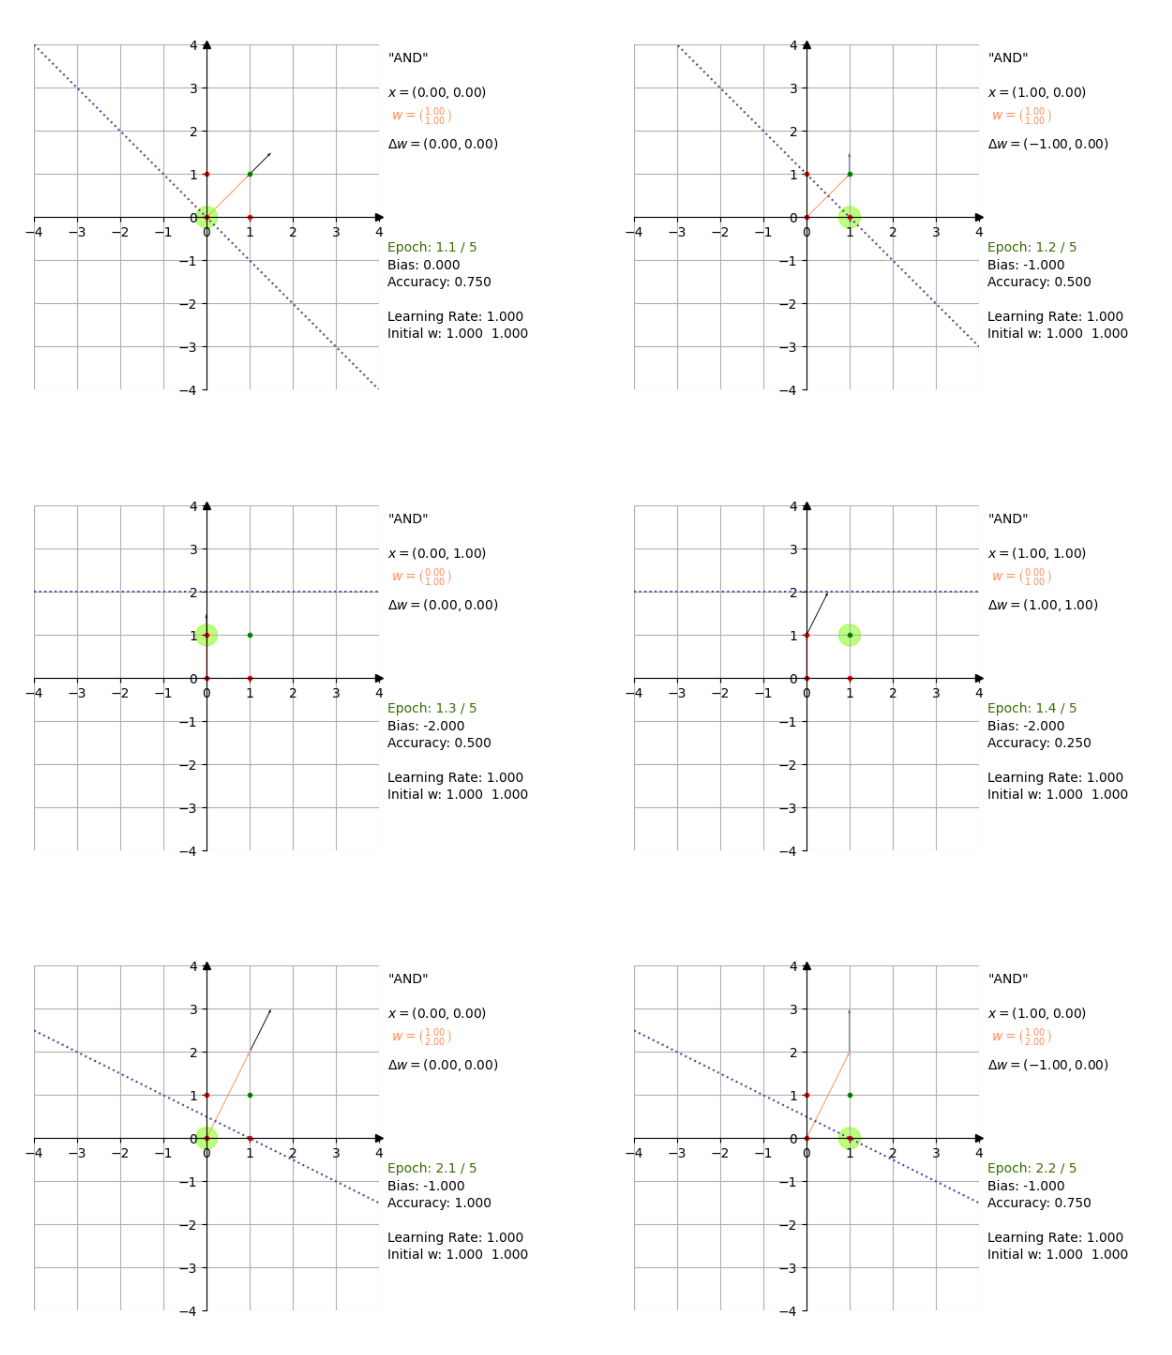
\includegraphics[
        width=18cm,
        keepaspectratio,
    ]{chapters/Anhang/images/epochs_1}
\end{figure}


\begin{figure}[h]
    \hspace*{-1cm}
    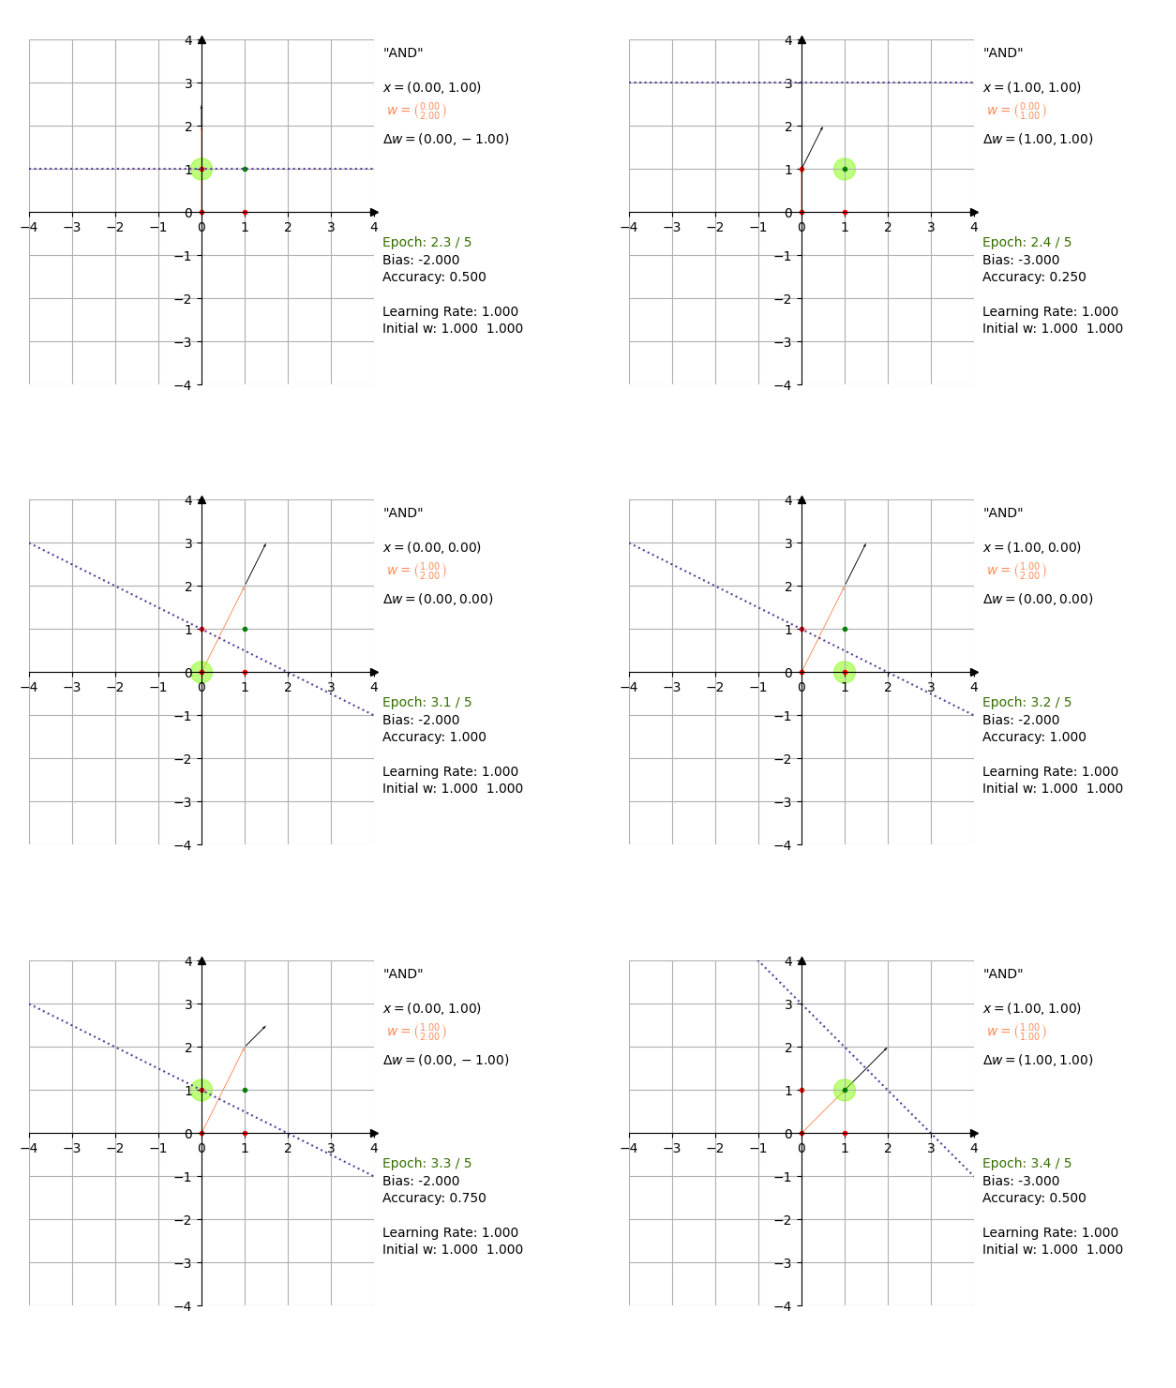
\includegraphics[
        width=18cm,
        keepaspectratio,
    ]{chapters/Anhang/images/epochs_2}
\end{figure}


\begin{figure}[h]
    \hspace*{-1cm}
    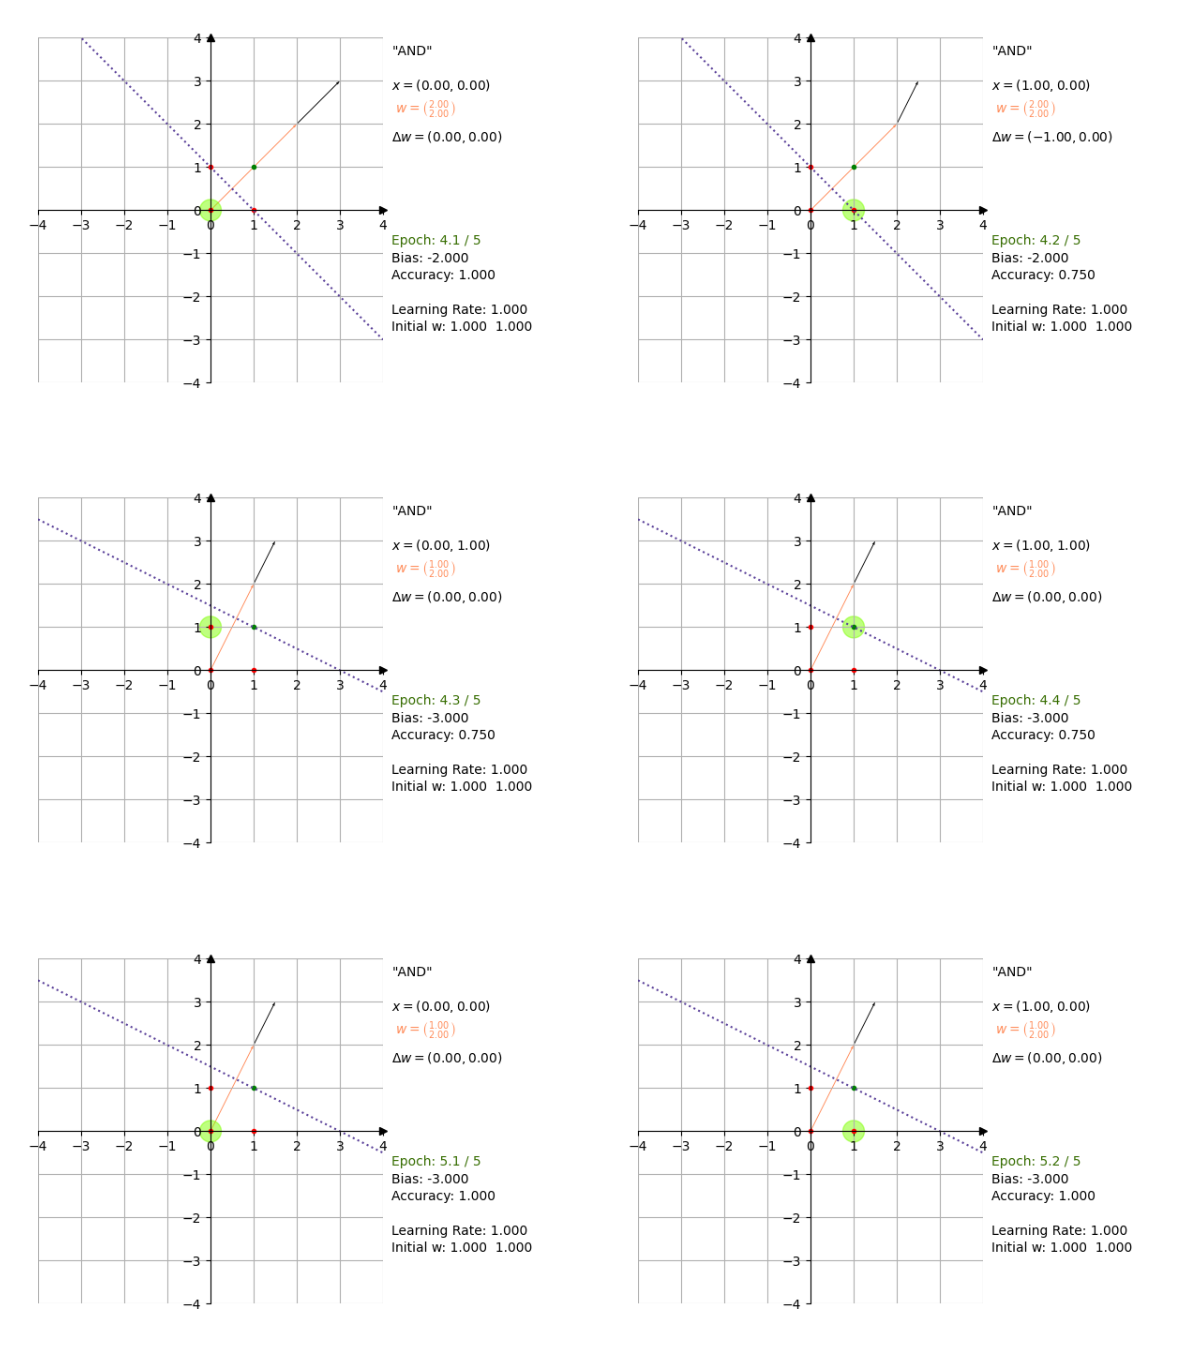
\includegraphics[
        width=18cm,
        keepaspectratio,
    ]{chapters/Anhang/images/epochs_3}
\end{figure}

\begin{figure}[h]
    \hspace*{-1cm}
    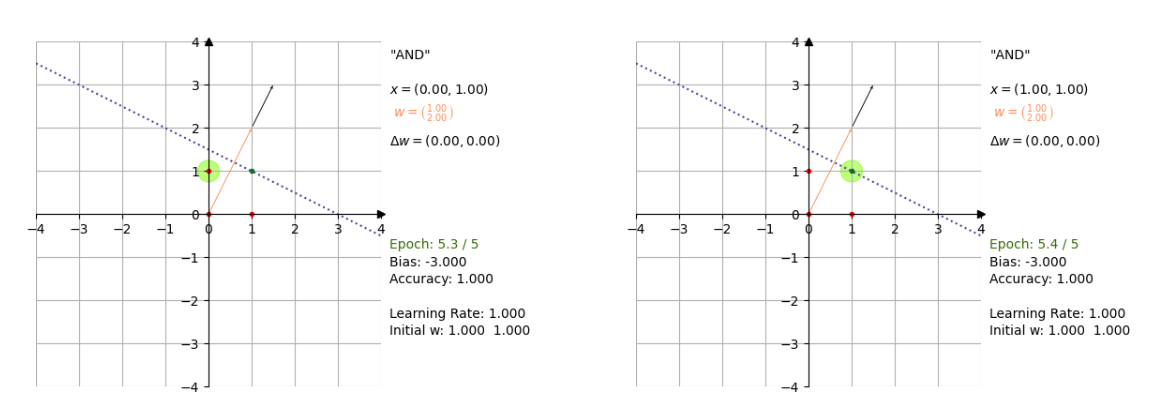
\includegraphics[
        width=18cm,
        keepaspectratio,
    ]{chapters/Anhang/images/epochs_4}
    \caption{Geometrische Darstellung der Konvergenz eines Perzeptrons für AND (Quelle: Eigene Darstellung)}
    \label{fig-rp-and-epochs}
\end{figure}